% ****** Start of file apssamp.tex ******
%
%   This file is part of the APS files in the REVTeX 4.2 distribution.
%   Version 4.2a of REVTeX, December 2014
%
%   Copyright (c) 2014 The American Physical Society.
%
%   See the REVTeX 4 README file for restrictions and more information.
%
% TeX'ing this file requires that you have AMS-LaTeX 2.0 installed
% as well as the rest of the prerequisites for REVTeX 4.2
%
% See the REVTeX 4 README file
% It also requires running BibTeX. The commands are as follows:
%
%  1)  latex apssamp.tex
%  2)  bibtex apssamp
%  3)  latex apssamp.tex
%  4)  latex apssamp.tex
%
\documentclass[reprint]{revtex4-2}

\usepackage{graphicx}% Include figure files
\usepackage{dcolumn}% Align table columns on decimal point
\usepackage{bm}% bold math
%\usepackage{hyperref}% add hypertext capabilities
%\usepackage[mathlines]{lineno}% Enable numbering of text and display math
%\linenumbers\relax % Commence numbering lines

%\usepackage[showframe,%Uncomment any one of the following lines to test 
%%scale=0.7, marginratio={1:1, 2:3}, ignoreall,% default settings
%%text={7in,10in},centering,
%%margin=1.5in,
%%total={6.5in,8.75in}, top=1.2in, left=0.9in, includefoot,
%%height=10in,a5paper,hmargin={3cm,0.8in},
%]{geometry}
\usepackage[pdftex, pdftitle={Article}, pdfauthor={Author}]{hyperref} % For hyperlinks in the PDF
\usepackage{float}

\begin{document}

\preprint{APS/123-QED}

\title{The SYK Model and Non-Fermi Liquids}% Force line breaks with \\


\author{Jash Desai}
\email[Correspondence email address: ]{jash_desai@brown.edu}% Your name
    \affiliation{Brown University, Department of Physics, Providence, RI}

\date{\today}% It is always \today, today,
             %  but any date may be explicitly specified

\begin{abstract}
This review paper is a broad overview of the phenomenon surrounding certain non-Fermi liquids and how these effects may be better understood via the use of the Sachdev-Ye-Kitaev (SYK) model. We discuss: how traditional Fermi-liquid theory breaks down in certain systems, the details of the SYK model, and the low and high energy limits of the SYK model. We are able to show the SYK model shows promise as a way to describe non-Fermi behavior. 
\end{abstract}

%\keywords{Suggested keywords}%Use showkeys class option if keyword
                              %display desired
\maketitle

%\tableofcontents

\section{\label{sec:level1}Introduction}
Quantum many-body problems have been at the heart of physics since their formulation. Since its introduction in 1956 \cite{Landau:1958joj}, Fermi-liquid theory has been a successful model for describing the limited case of  fermionic many-body problems. The theory describes properties of interacting fermions in metals and semiconductors by treating them as quasiparticles that behave similarly to non-interacting particles but with modified characteristics due to interactions. 
\par Fermi-liquid theory, however, has its limits in, among other points, low dimensional metals as well as systems with extremely strong interactions. Once Fermi-liquid theory reaches its descriptive limits in these instances, a system is referred to as a non-Fermi liquid. Several modern systems have non-Fermi liquid behaviour such as La$_{2-x}$Sr$_{x}$CuO$_{4}$ \cite{Takagi_1992}and BaFe$_{2}$(As$_{1-x}$P$_{x}$)$_{2}$\cite{Hayes_2016}. 
\par A possible model to combat the typical issue with modeling certain non-Fermi liquids has emerged via the collaboration of Sachdev, Ye, and Kitaev \cite{PhysRevLett.70.3339}\cite{Kitaev_2015}, known as the SYK model. The model is built from several promising axioms which help combat the issues which are encountered through standard investigative techniques. The model proposes randomly coupled Marjorana fermions in the Hamiltonian along with random interaction terms. Analysis of the SYK model at the low and high energy limits show promise of a strong ability to describe non-Fermi liquid type behavior in several instances. 
 

\section{Non-Fermi Liquids}
Fermi liquid theory can be described via a many-body Green's function as follows \cite{Girvin_Yang_2019}:
\begin{equation}
    G(\omega, p) \approx \frac{Z}{\omega + \mu - \epsilon(p)}
\end{equation}

We use the language of Green's functions to underscore the point that quasiparticles come from the analysis of the poles of this function and the propagation of single-particle excitations in the system. The Green's function in Fermi liquid theory takes into account the interactions between the particles and provides a way to describe the system in terms of effectively non-interacting quasiparticles. 
\par Fermi liquid theory has many distinguishing characteristics, including quadratic scaling of specific heat at low temperature scales, $C_{v} \approx T^{2}$ and heavy quasiparticle presence at phase transitions. However, in recent investigations of materials, several systems seem to break these rules and instead exhibit behaviors outside this model, we call these non-Fermi liquids.
\par We use experimental measurements to show these phenomenon such as linear resistivity in BaFe$_{2}$(As$_{1-x}$P$_{x}$)$_{2}$\cite{Hayes_2016}.
\begin{figure}[H]
    \centering
    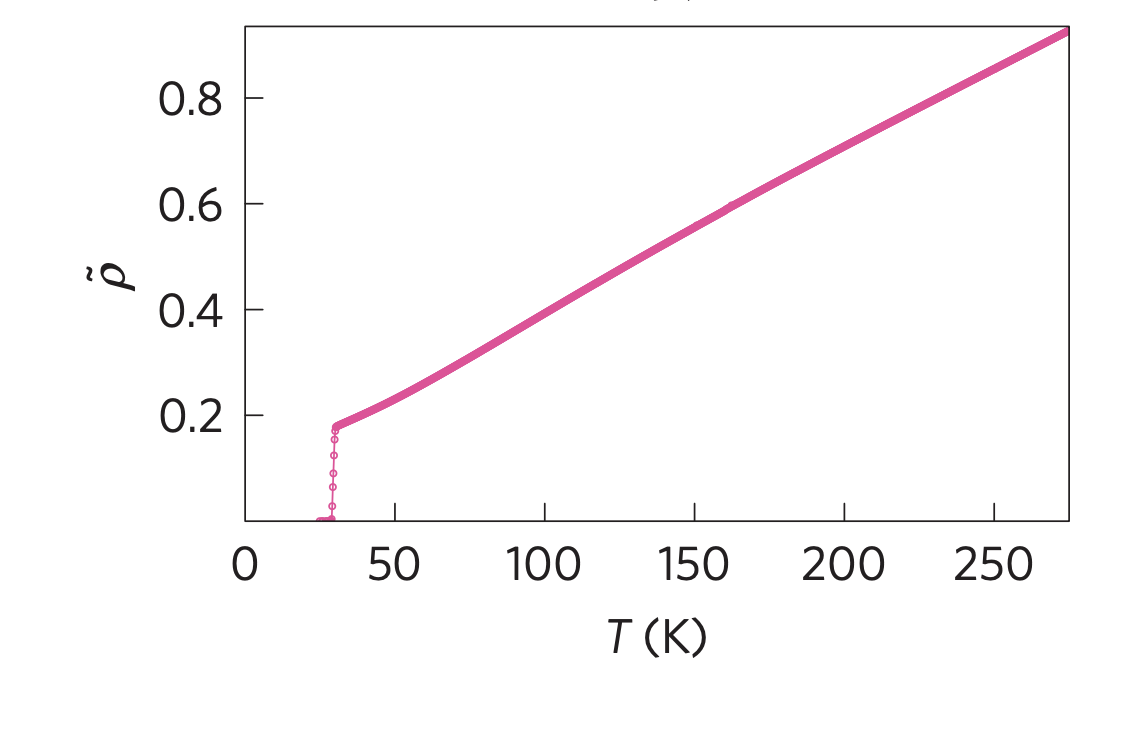
\includegraphics[scale = 0.4]{Linear.png}
    \caption{From \cite{Hayes_2016}. A modern metal with linear in temperature resistivity. Breaks the Fermi-liquid approximation.}
    \label{fig:enter-label}
\end{figure}

Additionally, we find "strange metals" which are Fermi liquid compliant until they phase transition in lower temperatures and exhibit non-Fermi behavior, YbRh$_{2}$Si$_{2}$ measured by Trovarelli, et. al is such an example \cite{PhysRevLett.85.626}. These strange metals also have potential spin-glass transitions if they are doped. Subsequently, many of these non-Fermi liquids exhibit signs of some form of spontaneous symmetry breaking at low energies as seen by Tatsumi and Sato \cite{Tatsumi_2009}.
\par These clues will help guide a suitable replacement for these unmet needs of Fermi-liquid theory: linear resistivity, some form of symmetry breaking at low energies, and characteristics of strange metals. 


\section{The SYK Model}
\subsection{The Random Matrix Model}
We begin the construction of the SYK model by motivating its intent via a simple model of a metal. More specifically, we imagine a simple metal with quasiparticles \cite{Sachdev_2023}. For the sake of simplicity, we assume that we don't need to keep track on any extraneous conservation laws and that the electrons in the model may move randomly between sites, one by one. Given these random sites movements, we would also expect random amplitudes. This leads us the random matrix model of a simple metal, originally posited by Bohigas, Giannoni, and Schmidt \cite{Bohigas_1984} and formalized by Müller, et al. \cite{Muller_2009}. We introduce the Hamiltonian for such as system in which electrons, $c_i$, hop between sites labeled $i = 1 \cdots N$, with a matrix element mediating the hopping, $t_{ij} / \sqrt{N}$. 
\begin{equation}
H_{2} = \frac{1}{(N)^{1/2}}\sum_{i,j =1}^{N} t_{ij}c_{i}^{\dagger}c_{j} -  \mu \sum_{i}c_{i}^{\dagger}c_{i}
\end{equation}

In which the electron-electron interactions are mediated by the following commutation relations:
\begin{equation}
    \{c_{i},c_{j}\} = 0
\end{equation}
    
 
\begin{equation}
    \{c_{i},c_{j}^{\dagger}\} = \delta_{ij}
\end{equation}

In order to find the solution to the spectrum of eigenstates for this model, we simply numerically diagonalize the $N \times N$ matrix for $t_{ij}$. The novelty of such a simple solution to the random matrix model is that when this technique is carried out in the limit of large N, certain quantities the model predicts, e.g. energy eigenvalues, hopping energy,  are self-averaging. Therefore, given some material's sample $t_{ij}$, we can infer that as $N \rightarrow \infty$, those quantities' values converge to one, to their averaged value over all samples \cite{Chowdhury_2022}.
\par The (energy corrected) Green's function for a single-particle energy also informs us to an important similarity to Fermi-liquid theory. Due to its solvable nature, originally done in a nuclear physics context by Weidenmuller and Mitchell \cite{Weidenm_ller_2009}, the poles exhibit a simple structure which points to the existence of quasiparticles in this model, a feature which links it to Fermi-liquid theory.
\begin{equation} \label{eq:4}
    G(\epsilon, i \omega_{n}) = \frac{1}{i\omega_{n} + \mu + \epsilon}
\end{equation}
\begin{figure}
    \centering
    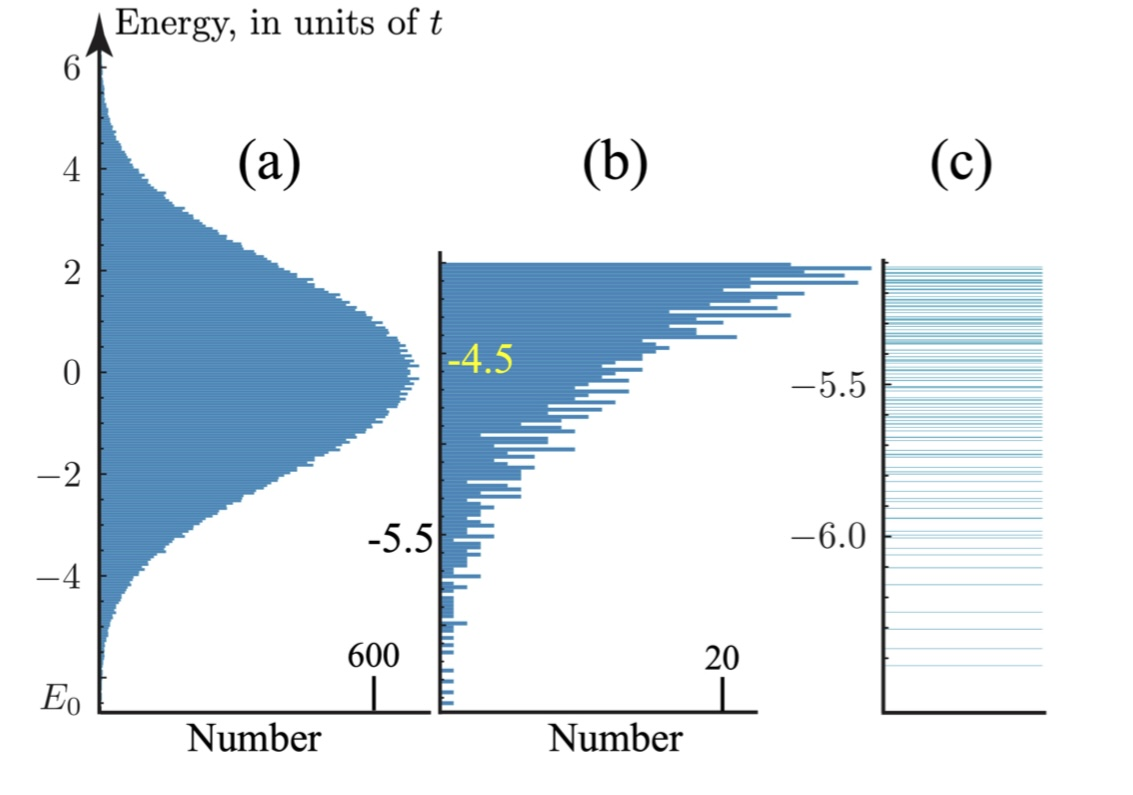
\includegraphics[scale = 0.4]{RandomMatrixSpectrum.jpeg}
    \caption{From \cite{Chowdhury_2022}, we have the many-body eigenvalues for N = 32 random matrix model. $\mathcal{N}$(E) is graphed out in (a) and (b) while (c) is the individual energy levels.}
    \label{Fig1}
\end{figure}

The Gaussian output of the energy eigenvalues, per Fig. 1, the model conforms to a normalized behavior of the excited quasiparticles. This leads to three key observations of the random matrix model: the model is able to capture a great deal of system that may be modeled by quasiparticles, the final analysis of the energy eigenvalues show that the model is limited to well-behaved excitations and is unable to capture more chaotic or long-range behaviour, and finally, system specific features (e.g. strong correlations) cannot be captured via the Gaussian.
\par While the use of quasiparticles in the random matrix model provides a natural extension to Fermi-liquid theory, we find that there are still massive restrictions in the ability of such models to encompass all types of disordered behaviours. This is where we may use the SYK model to investigate these anomalies. 
\subsection{The SYK Model}
We introduce the Hamilonian for the SYK model, formalized after corrections of Kitaev \cite{Kitaev_2015}. 
\begin{equation}\label{eq:5}
    H_{4} = \frac{1}{(2N)^{3/2}} \sum_{ijkl =1}^{N} U_{ijkl} c_{i}^{\dagger}c_{j}^{\dagger}c_{k}c_{l} -  \mu \sum_{i}c_{i}^{\dagger}c_{i}
\end{equation}

We notice that the Hamiltonian for the SYK model is very similar to the random matrix model with a few key exceptions. Firstly, while the random matrix model had a hopping term for a one particle interaction, the SYK model posits random couplings of two particles, via $U_{ijkl}$. The couplings themselves are independent random variables such that they satisfy the following conditions:

\begin{equation}
       \overline{U_{ijkl}} = 0 
\end{equation}
\begin{equation}
      U_{ij;kl} = -U_{ji;kl} = -U_{ij;lk} = U^{\star}_{kl;ij}    
\end{equation}
We also introduce the relevant commutation relations. In this case, due to the introduction to two particle states, our commutation relations maintain the same general conditions for a two particle limiting case, but the relation for all particle states between the Majorana fermions may be generalized as Eq. \ref{eq.10} shows. This generalization was done via the work of \cite{Polchinski_2016}.
\begin{equation}
    \{c_{i},c_{j}\} = 0
\end{equation}
\begin{equation}
    \{c_{i}, c_{j}^{\dagger}\} = \delta_{ij}
\end{equation}
We may state that for all Majorana fermionic interactions, the generalized relation is a Clifford relation.
\begin{equation} \label{eq.10}
    \{c_{i}, c_{j}\} \rightarrow \{\psi_{i}, \psi_{j}\} = 2\delta_{ij}
\end{equation}
To understand the power of the SYK model, we immediately turn to the many-body Green's function and notice a distinct difference between it and Eq. \ref{eq:4}. We derive the Green's function from these "melon" diagrams motivated by the calculation of an electron self energy, $\Sigma(\tau)$,  or the energy an electron has as a result of changes it causes in vaccua. This was generalized to a large $N$, Majorana fermion case by Klebanov and Tarnopolsky \cite{Klebanov_2017}. 
\begin{figure}[H]
    \centering
    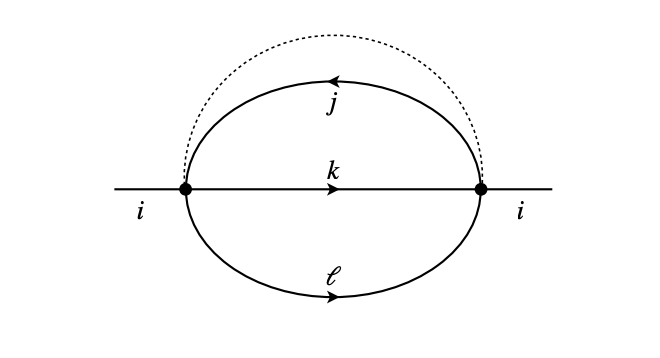
\includegraphics[scale = 0.7]{Melon Diagram.png}
    \caption{From \cite{Klebanov_2017}. This melon diagram describes a simple interaction between the proposed 4 Majorana fermions in the SYK Hamiltonian. The solid lines reprsent single particle Green's functions while the dashed line represent an average disordered state with the interactions between the fermions. Said interactions average out to $\overline{U_{ijkl}}^{2}$ }.
    \label{fig:2}
\end{figure}
The analysis of said field diagram leads to follwing set of non-linear Green's functions, with a self-energy boundary condition:
\begin{equation}
    G(i\omega_{n}) = \frac{1}{i\omega_{n} + \mu - \Sigma(i\omega_{n})}
\end{equation}
\begin{equation}
    \Sigma(\tau)= -U^{2}G^{2}(\tau)G(-\tau)
\end{equation}
\begin{equation}
    G(\tau = 0) = \mathcal{Q}
\end{equation}
Very much unlike Eq. \ref{eq:4} for the random matrix model, there is no analytic solution for this Green's function, due to the non-linear interactions, and thus we are forced to take limits to glean further insight into relevant observables such as density of states or energy eigenvalues. Despite there being little insight into observables, the analysis of Witten \cite{Witten:2016iux} informs us to an extraordinary difference between the SYK model and the random matrix model. That being, when analyzing the Green's function, we find that it contains a branch cut singularity along with a non-trivial frequency dependence in the self-energy. This indicates to us that the SYK model does not have quasiparticles as Fermi-liquid theory and the random matrix model does.
\par  When analyzing the graphed energy eigenvalues of the SYK model via numerical analysis in Fig. \ref{fig:3}, we find a distribution that looks distinctly different from the random matrix model in Fig \ref{Fig1}.
\begin{figure}
    \centering
    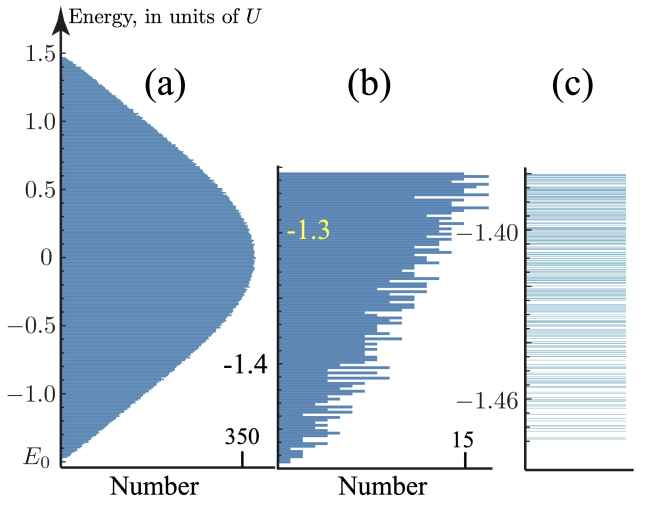
\includegraphics[scale = 0.6]{SYK Spectrum.png}
    \caption{From \cite{Chowdhury_2022}. The many-body eigenvalues of a $N$ = 32 Majorana SYK Hamiltonian. $\mathcal{N}$(E) is plotted in (a) and (b) while (c) shows the band energies.}
    \label{fig:3}
\end{figure}
The distribution for the SYK Hamiltonian shows an energy eigenspectra that has far greater kurtosis and heavy-tailed groupings than the random-matrix model did. This leads us to believe the SYK model accounts for a greater amount of interactions and excited states than random-matrix model could. Furthermore, when analyzing the band spacing, we find a sparser spacing $\approx 1/N$ at the bottom of the band for the random matrix model. This gives us another hint as to the chaotic nature of the model. 
\par We find that the denser band spacing is due to high degree of level repulsion in the energy spectrum, leading to more rigid spacing. This is seen as a sign of strong correlations, a characteristic feature of many non-Fermi liquids and something the SYK model embeds within itself. \cite{Orman:2024mpw}. 
\par Given these hints as to the more holistic nature of the SYK model in capturing more phenomenon, we may look at the limit driven analysis (in particular, the low energy limit) to find closer connections to non-Fermi liquids and phenomenon. 


\section{Applications of the SYK model to Non-Fermi Liquids}
\subsection{The Low Energy Limit of the SYK Model }
We leave the technical analysis of the low energy limit in the Appendix and in the capable hands of Louw, van Manen, and Jha \cite{Louw:2023lpq}. 
\par The low energy limit for the SYK model is set at a frequency far below the charateristic energy scale of the model, $|\omega| << J$. As such, the Green's function takes the form:
\begin{equation}\label{eq:14}
    G(\omega) \approx \frac{1}{J}(\frac{|\omega|}{J})^{-1/q}
\end{equation}
While the self-energy term scales as: 
\begin{equation}
    \Sigma(\omega) \approx J(\frac{|\omega|}{J})^{1-\frac{2}{q}}
\end{equation}
In which $q$ is the number of Majorana fermions involved in each interaction term. Per these expressions we may glean a few characteristics of the low energy limit of the SYK model.
\par Firstly, we note that the low energy expressions have changed from non-linear in the frequnecy domain to linear. This points to an important sign that all frequency dependent may now scale differenlty than they did before the low-energy limit was taken. Before further mathematical analysis, we can simply consult a numerical analysis of the scaling terms in background of a quantum critical metal with spin-1/2 fermions by Cha, Wentzell, Parcollet, Geroges, and Kim \cite{Cha_2020}. 
\par While Cha, et al. used a slighlty different SYK Hamiltonian than the more general expression given in Eq. \ref{eq:5}, the same procedure was taken to find the relevant low energy limit with an analytic continuation made for the Green's function to recover Eq. \ref{eq:14}. 
\begin{figure}[H]
    \centering
    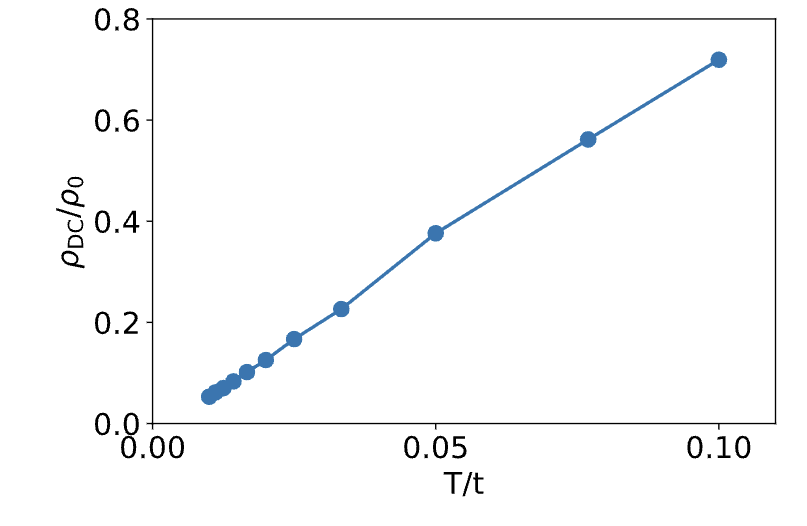
\includegraphics[scale = 0.6]{SYKLinear.png}
    \caption{From \cite{Cha_2020}. Resistivity $\rho_{DC}/\rho_{0}$ vs. temperature $T/t$ computed via analytic continuation of Green's function.}
    \label{fig:4}
\end{figure}
Fig. \ref{fig:4} shows one of the primary signs of a non-Fermi liquid as previously discussed at the beginning of this article, a linear specific-heat scaling that can only be found in non-Fermi liquids. This follows from our initial intuition about the low energy expressions we derived and we now have proof of said argument via a quantum-critical metal as a toy model.
\par We may further probe this low-energy limit of the SYK model via a supersymmetric (SUSY) version to further see non-Fermi liquid like behavior. Using the SUSY model introduced by Fu, Gaiotto, Maldacena, and Sachdev \cite{Fu_2017}, we are able to find the conformal symmetry of the model. 
\par Per Fu, et. al's analysis of the $\mathcal{N} = 2$ version of the SUSY SYK, the recovered relation between the low energy Green's functions and the reparametrization symmetry of the model is as follows:
\begin{equation}
    G_{b\overline{b}} \ast G_{\overline{\psi}\psi}^{\hat{q} - 1} = - \delta
\end{equation}
\begin{equation}
    G_{\psi \overline{\psi}} \ast [(\hat{q} - 1)G_{\overline{b},b}G_{\overline{\psi}\psi}^{\hat{q}-2}] = -\delta
\end{equation}
The above relations, in which $b$ and $\psi$ respectively stand for any pair of bosons (bosons are introduced into the SYK model via SUSY see \cite{Maldacena_2016} for further details) and Majorana fermions with complex conjugates, we find that reparametrization symmetry in the SYK model has been broken via a static anomaly, $- \delta$.
\par This symmetry breaking gives rise to a so called "Schwarzian mode" which dominates the low-energy dynamics of the model. This is yet another indicator of a non-Fermi liquid behavior in the low-energy limit, as we previously mentioned in the discussion regarding Tatsumi and Sato \cite{Tatsumi_2009}. 
\par Another extension of this Schwarzian mode as an indicator of non-Fermi liquid argument can be found in Haldar, Banerjee, and Shenoy's \cite{Haldar_2018} investigation of a higher dimensional SYK model placed in a lattice which finds this Schwarzian mode at a Lifshitz transition, a change in the topology of the Fermi surface which results in spontaneous symmetry breaking and, in this case, a transition to a non-Fermi liquid. A similar observation is made by Kitaev and Suh in their analysis of the SYK model and its gravitational dual \cite{Kitaev_2018}.
\par The observation of linear specific heat scaling and Schwarzian mode domination at low energies provides compelling evidence that the low energy limit of the SYK model is well suited to describe non-Fermi liquid behavior in several systems. We now move to the high energy or $N \rightarrow \infty$ limit which has its own peculiarities. 
\subsection{The $N \rightarrow \infty$ Limit of the SYK Model}

\par In the $N \rightarrow \infty$ limit of the SYK model, we find a Green's function and self energy expression of the following form, originally calculated by Fu and Sachdev \cite{Fu_2016}  with further corrections by Maldecena and Stanford \cite{Maldacena_2016}. We also impose (somewhat obviously from the last case) that $|\omega| >> J$. 
\begin{equation}
    G(\omega) \approx (\frac{1}{\omega})(\frac{J}{|\omega|})^{2/q}
\end{equation}
\begin{equation}
    \Sigma(\omega) \approx \omega(\frac{J}{|\omega|})^{2/q}
\end{equation}
These particular functions, while having intersting properties in their own right, don't reveal much about non-Fermi liquid behavior as they due other important characteristics of SYK at high energy such as thermalization or holographic duality [\cite{Jevicki_2016},\cite{Jevicki_2022}.Alas, these are out of the scope of this article. 
\par However, we may construct a strange metal which obeys these experimentally anomalies in a restricted case of two dimensions per the prescription of Song, Jian, and Balents. \cite{Song_2017}.
\begin{figure}[H] 
    \centering
    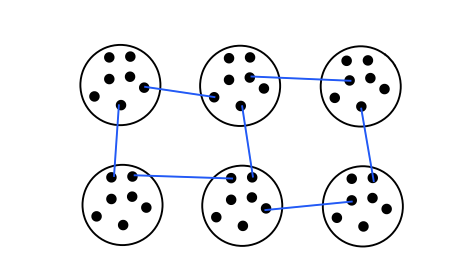
\includegraphics{SYKLattice.png}
    \caption{From \cite{Rosenhaus:2018dtp}. Simple representation of the way a lattice may be constructed via the SYK model. The lattice is made up of SYK quantum dots with random interactions between dots.}
    \label{fig:5}
\end{figure}
We present a visual representation of what Song et. al do with the SYK interactions in Fig. \ref{fig:5}. By creating a lattice of $N$ SYK islands and then turning on the random interactions such that when $N$ fermion modes are pushed to $N \rightarrow \infty$, we recover a strongly correlated metal with strange metal phase transitions.
The construction from Song et. al uses the same quartic Majorana fermion Hamiltonian we presented in Eq. \ref{eq:5}. 
\par Some items of interest to note are the linear in temperature resistivity up until a phase transition into the Fermi liquid regime and heavy quasiparticle presence in the Fermi liquid range. Additionally in Fig \ref{fig:6}., as $\mathcal{T} \rightarrow \infty $, the entropy and specific heat collapse to universal functions of $\frac{T}{E_{c}}$, that is, at fixed $\frac{T}{E_{c}}$, we find conformal behavior, a property of non-Fermi liquids and, subsequently, strange metals. 
\begin{figure}[H]
    \centering
    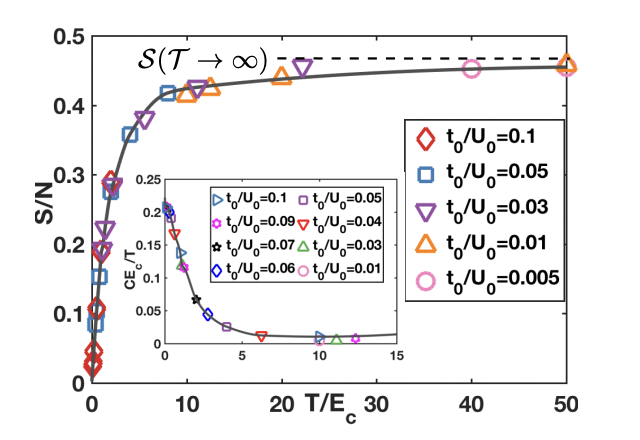
\includegraphics[scale = 0.8]{StrangeMetal.png}
    \caption{From \cite{Song_2017}. Entropy and specific heat correlations of the constructed strange metal with fixed $\frac{T}{E_{c}}$}
    \label{fig:6}
\end{figure}
\par While the high energy limit of the SYK model lends itself to more theoretical applications, in particular for black holes and quantum gravity [\cite{PhysRevX.5.041025}\cite{Sachdev:2022qnu}\cite{Sachdev:2023try}], it also provides a playground for the use of the SYK model as a soluble source of strong local interactions which reproduces a remarkable number of features of strongly correlated metals, albeit with very theoretical conditions. 
\section{Conclusion}
We finish this review article with the following key takeaways about the SYK model: 
\begin{itemize}
    \item Non-Fermi liquids have become an important part of modern condensed matter physics due to their exotic physics and deviation from standard Fermi liquid theory. 
    \item Fermi-liquid theory's use of quasiparticles hold it back from modeling several disordered and strongly correlated systems including non-Fermi liquids and strange metals.
    \item The random matrix model is able to reconstruct much of Fermi-liquid theory's range of interaction description without the explicit use of quasiparticles via random Fermionic couplings.
    \item The SYK model can go beyond the random matrix model with the use of random interactions and couplings with a quartic Majorana fermion model. The SYK model does not have quasiparticles.
    \item When juxtaposing the energy eigenvalues of the random matrix model and the SYK model, the SYK model accounts for a larger range of interactions including strong correlations and long-range interactions. 
    \item The low-energy limit of the SYK model recovers non-Fermi behavior such as linear resistivity and a Schwarzian mode that dominates low-energy dynamics due to reparametrization of symmetry breaking. 
    \item The high energy limit links the SYK model to black holes and thermofield calculations but also allows for the SYK model to be constucted as a working example of a strange metal.
\end{itemize}
The SYK model has become an invaluable part of modern condensed matter and modern high energy theory due to its flexibility and connections to random matrix theory. While there were a number of topics of not discussed here including quantum simulations, zero-temperature entropy, and a deep dive into tensor models of the SYK model, this small focus on non-Fermi liquids displays the SYK model's utility. 
\begin{acknowledgments}
This project was part of PHYS2420 under Dr. Kemp Plumb and wouldn't be possible without his feedback and subsequent discussion on the topic. A special thanks to Dr. Antal Jevicki for relevant discussions. 

\end{acknowledgments}


% The \nocite command causes all entries in a bibliography to be printed out
% whether or not they are actually referenced in the text. This is appropriate
% for the sample file to show the different styles of references, but authors
% most likely will not want to use it.


\bibliography{bibliography}% Produces the bibliography via BibTeX.

\end{document}
%
% ****** End of file apssamp.tex ******

